\section{Modello di Ising 2D}

Il modello di Ising 2D consiste in un reticolo quadrato bidimensionale di spin, i quali possono assumere solamente i valori 
$\pm 1$. Nel limite termodinamico, tale modello presenta una transizione di fase in prossimità di una temperatura critica Tc.
Per $T\,>\,Tc$ il sistema si comporta in modo paramagnetico, altrimenti si ha una magnetizzazione spontanea, evidenza 
di ordine nel reticolo di spin. Il modello presenta soluzione analitica solamente con campo magnetico nullo $h\,=\,0$, 
determinata da Onsager nel 1944. La magnetizzazione 

\begin{equation}
    m\left(\beta,\,h=0\right)\,=\,
    \begin{cases}
    \left[1\,-\,\dfrac{1}{\sinh^4{\left(2\beta J\right)}}\right]^{\frac{1}{8}} \qquad \qquad T\,<\,T_c \\
    0 \qquad \qquad \qquad \qquad \qquad \qquad \,\,\,\, T\,>\,T_c
    \end{cases}
    \label{eq: magn_Onsager_1944}
\end{equation}
presenta una discontinuità alla temperatura critica 

\begin{equation}
    T_c\,=\,\frac{2J}{\ln{\left(1\,+\,\sqrt{2}\right)}}\,,
    \label{eq: tc_Ising2D_Ons}
\end{equation}
evidenza ulteriore di una transizione di fase.


\subsection{Domain walls}

Mentre il modello di Ising 1D non presenta transizione di fase a temperatura finita, nel modello di Ising 2D è possibile la manifestazione 
di ordine a lungo raggio al di sotto di una certa temperatura critica $T_c$. Consideriamo ora il mapping riportato in Figura 
\ref{fig: map_2to1_Ising}, in cui i siti reticolari di un modello bi-dimensione vengono mappati su una catena lineare (mantendo 
l'interazione con i primi vicini di partenza).

\begin{figure}[H]
    \centering
    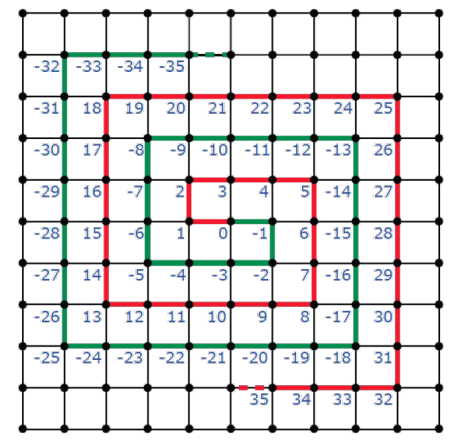
\includegraphics[width=0.5\textwidth]{Immagini/map_2to1_Ising.png}
    \caption{Mapping di un modello di Ising 2D su un modello di Ising 1D. Immagine da \cite{galliFSA}.}
    \label{fig: map_2to1_Ising}
\end{figure}

Sebbene si possa mappare il reticolo quadrato in una catena di spin, il motivo per cui tale reticolo lineare è ordinato a temperatura 
finita è da ricercare nel range dell'interazione. Nel caso del modello di Ising 1D con interazione fra primi vicini, la stessa è short 
range, poichè coinvolge solamente i siti adiacenti a quello preso in considerazione. Nel caso invece di catena di spin ottenuta come 
risultato del mapping di un reticolo quadrato in uno lineare, l'interazione è long-range, ed a ogni nuovo cambio di direzione delle 
spirali concentriche con cui si visitano tutti i siti reticolari tale lunghezza d'interazione aumenta. Nel caso della catena di 
spin ottenuta a partire da un reticolo quadrato anche i domain walls interagiscono fra loro con un potenziale di tipo long-range, andando 
ad invalidare il discorso fatto in precedenza e rendendo possibile una magnetizzazione non nulla anche per una catena di spin. 

\subsection{Scale free fenomena}


